% arara: pdflatex: {interaction: nonstopmode, synctex: on,  shell: yes}
% arara: bibtex if found('log', 'Citation .* undefined')
% arara: pdflatex: {interaction: nonstopmode, synctex: on,  shell: yes}  if found('log', 'undefined references') or found('log', 'Rerun to') or found('log', 'Citation .* undefined')
% arara: pdflatex: {interaction: nonstopmode, synctex: on,  shell: yes}  if found('log', 'Rerun to') or found('log', 'Citation .* undefined')

\documentclass{cubeamer}
\input macros.tex
\input tikz.tex
\input acronyms.tex
\usetikzlibrary{positioning}
%%% Custom TikZ addons
\usetikzlibrary{crypto.symbols}
%\tikzset{shadows=no}  
\usetikzlibrary{decorations.pathreplacing}
\usetikzlibrary{arrows}
\usetikzlibrary{arrows.meta}
\usetikzlibrary{patterns}
\usetikzlibrary{shapes}
\usetikzlibrary{shadows}
\usetikzlibrary{calc}
\usetikzlibrary{math}

\hypersetup{
    colorlinks=true,
    linkcolor=blue,
    citecolor=green,
    urlcolor=cyan
}
\def\makethanks{%
    \begin{frame}
        \frametitle{\thankstitle}
        \thanksmessage
    \end{frame}
}
% in ``article'' mode there's no ``Thank you'' page
\mode<article>
{\providecommand\makethanks{}}


% commands for the title and message of the "Thank you" page
\def\thankstitle#1{\def\thankstitle{#1}}
\def\thanksmessage#1{\def\thanksmessage{#1}}
\thankstitle{}
\thanksmessage{{\huge {\color{red} Thank You} for your attention!} \\ \Large Any questions?}


\title[Key Recovery Attack on \texttt{FEAT\_PACQARMA3}]{Key Recovery Attack on \texttt{FEAT\_PACQARMA3} Feature}
% \subtitle{\green{National Workshop on Cryptology 2025, IIT Bhilai}}
\author[\red{Shibam}]{Roberto avanzi
    \and Orr Dunkelman
    \and \red{Shibam Ghosh}$^1$
}
% \date{\today} % or whatever the date you are presenting in is
\date{January 29, 2026} % or whatever the date you are presenting in is
\institute[IIT Hyderabad]{$^1$\textcolor{redd}{Department of CSE, IIT Hyderabad}}
% \institute[INRIA, Paris]{INRIA, Paris, France}

 \AtBeginSection[] { %
    \begin{frame}[noframenumbering]
        \frametitle{Plan of this Section}
        \tableofcontents[
        currentsection,
        currentsubsection,
        sectionstyle=show/shaded,
        subsectionstyle=show/show/hide,
        subsubsectionstyle=hide]
    \end{frame}
}

% --- Frametitle Customization ---

% % 1. Define your professional blue color (using RGB values)
% \definecolor{professionalblue}{RGB}{0, 90, 156} % A nice, deep corporate blue

% % 2. Set the frametitle colors
% \setbeamercolor{frametitle}{
%   fg=professionalblue,  % fg = foreground (the text color)
%   bg=normal text.bg     % bg = background (matches the slide background, effectively removing the shade)
% }
% % --- Remove the headline (progress bar) ---
% \setbeamertemplate{headline}{}


\tcbuselibrary{many}
% \usepackage[many]{tcolorbox}
\setbeamertemplate{itemize item}{$\blacktriangleright$}
\setbeamertemplate{itemize subitem}{$\triangleright$}
\setbeamertemplate{itemize subsubitem}{$\rhd$}

% Later, reload hyperref with your desired options:
\hypersetup{
    colorlinks=true,
    linkcolor=blue,
    citecolor=green,
    urlcolor=cyan
}

% -------------------------------------------------------
% Define Cyan Color for Title
% -------------------------------------------------------
\definecolor{myctyan}{RGB}{0,180,200}
\definecolor{mytheme}{RGB}{0, 51, 102}
\definecolor{cardbg}{RGB}{235, 242, 252}  % Light blue tint
% -------------------------------------------------------
% Override Frame Title Template
% -------------------------------------------------------
\setbeamertemplate{frametitle}{
    \vspace{0.1cm}
    \textcolor{mytheme}{\Large\textbf{\insertframetitle}}
    \vspace{0.05cm}
}

% -------------------------------------------------------
% Remove Navigation Symbols
% -------------------------------------------------------
\setbeamertemplate{navigation symbols}{}

% -------------------------------------------------------
% Optional: Clean Footline
% -------------------------------------------------------
\setbeamertemplate{footline}{
    \begin{beamercolorbox}[wd=\paperwidth,ht=0.2cm,dp=0.2cm]{footline}
        \hspace{0.2cm}
        
\includegraphics[scale=0.1]{img/Inria.png}
        \hfill
        \textcolor{gray}{\tiny\insertframenumber\,/\,\inserttotalframenumber}
        \hspace{0.5cm}
    \end{beamercolorbox}
}

% ---- ADD THIS AT THE END OF YOUR PREAMBLE ----
\makeatletter
\beamer@frametopskip=0pt plus 0pt\relax       % No flexible space on top
\beamer@framebottomskip=0pt plus 1fill\relax  % All flexible space goes to bottom
\makeatother


\usepackage{etoolbox}
\makeatletter
% Remove top filler from frame body
\patchcmd{\beamer@calculateheadfoot}{\vfill}{}{}{}
\makeatother
% ----------------------------------------------

% Put this in your preamble

% Section slide
\AtBeginSection[]{
    \begin{frame}[plain, noframenumbering]
        \begin{center}
            \vfill
            \textcolor{myctyan}{\rule{0.6\textwidth}{1.5pt}}
            \vspace{0.3cm}

            \textcolor{myctyan}{\Huge\textbf{\insertsectionhead}}

            \vspace{0.3cm}
            \textcolor{myctyan}{\rule{0.6\textwidth}{1.5pt}}
            \vfill
        \end{center}
    \end{frame}
}

% Subsection slide
\AtBeginSubsection[]{
    \begin{frame}[plain, noframenumbering]
        \begin{center}
            \vfill

            % Show parent section in smaller text above
            \textcolor{myctyan!60}{\large\textbf{\insertsectionhead}}

            \vspace{0.3cm}
            \textcolor{myctyan}{\rule{0.4\textwidth}{0.8pt}}
            \vspace{0.3cm}

            % Show subsection in larger text below
            \textcolor{myctyan}{\LARGE\textbf{\insertsubsectionhead}}

            \vfill
        \end{center}
    \end{frame}
}


\begin{document}

\maketitle

\begin{frame}[t]
    \frametitle{Table of contents}
    \tableofcontents
\end{frame}
%\cutoc


\section{Arm's \texttt{FEAT\_PACQARMA3} Feature and Summary of the Target}

\begin{frame}
\frametitle{The Pointer Authentication Code (\textsf{PAC}) feature}

\begin{enumerate}
\item Introduced in \blue{Arm V8} architecture in 2016~\cite{ARMv8-A-2016-additions} for enforcing CFI
\begin{enumerate}
\item $\textsf{Tag} \gets \red{\textsf{PRF}}(\text{Return Address, Pointer’s Context Information}) $
\item Inserts tag on function entry in reserved bits of pointers and verifies it upon exit
\begin{figure}[t]
    \centering
    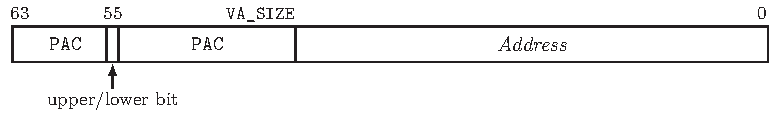
\includegraphics[scale=0.8]{./fig/pac-fields.pdf}
\end{figure}
\end{enumerate}
\pause
\item Discard some output bits of a \red{lightweight} Tweakable Block Cipher (TBC)
\pause
\item Protects against attacks targeting stack manipulation
\item \red{First line of defense} to system software and complex programs, e.g., Browsers

\end{enumerate}
\end{frame}
\begin{frame}
\frametitle{Block Cipher}
    \centering
    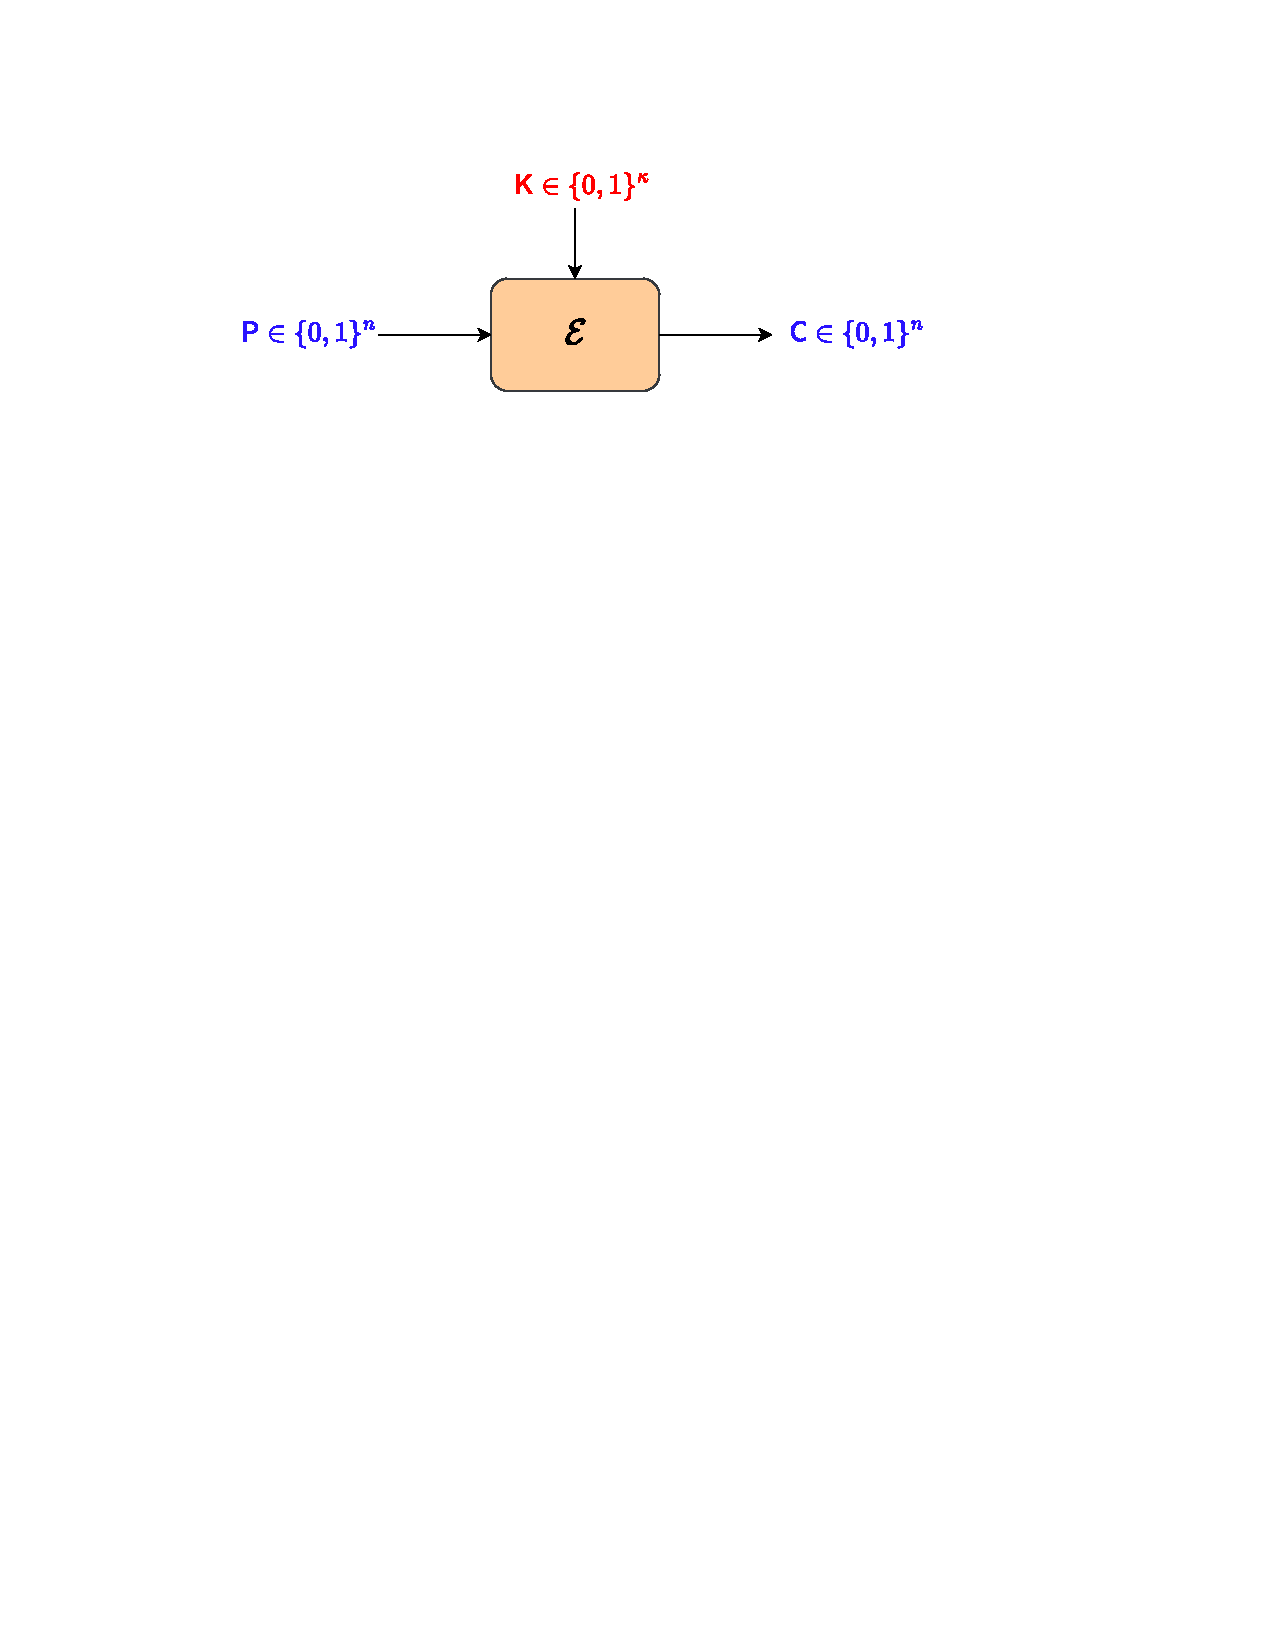
\includegraphics[width=17cm]{./fig/bc.pdf}
\end{frame}

\tikzset{
    blockcipher1/.style={
		fill=blue!10,
		rectangle,
		draw=bluee,
		semithick,
		inner sep=0pt,
		minimum height=1cm,
		minimum width=1cm,
		rounded corners=1mm,
	},
    blockcipher2/.style={
		fill=teal!10,
		rectangle,
		draw=green,
		semithick,
		inner sep=0pt,
		minimum height=1cm,
		minimum width=1cm,
		rounded corners=1mm,
	},
    roundfunction/.style={
		fill=blue!10,
		rectangle,
		draw=violet,
		semithick,
		inner sep=0pt,
		minimum height=1cm,
		minimum width=1cm,
		rounded corners=1mm,
	},
}

% Add to preamble
\newcommand{\drawAppTreeBase}{
    \useasboundingbox (-13, -8) rectangle (13, 5.5);

    % ROOT
    \node[app root, minimum width=5cm, minimum height=1.2cm,
          font=\Large\bfseries] (root)
        at (0, 4.5) {Low-Latency Cryptography};

    % Main horizontal connector
    \draw[thick, rootcolor] (0, 3.9) -- (0, 3.2);
    \draw[thick, rootcolor] (-8.5, 3.2) -- (9.5, 3.2);

    % All vertical drops
    \draw[thin, subcolor!25] (-8.5, 3.2) -- (-8.5, 2.4);
    \draw[thin, subcolor!25] (-3.0, 3.2) -- (-3.0, 2.4);
    \draw[thin, subcolor!25] (3.0, 3.2)  -- (3.0, 2.4);
    \draw[thin, subcolor!25] (9.5, 3.2)  -- (9.5, 2.4);

    % All branches dimmed by default
    \node[app branch dim, minimum width=4.2cm, minimum height=1cm,
          font=\normalsize] (mem)
        at (-8.5, 1.8) {Memory\\Encryption};
    \node[app branch dim, minimum width=4.2cm, minimum height=1cm,
          font=\normalsize] (code)
        at (-3.0, 1.8) {Code\\Encryption};
    \node[app branch dim, minimum width=4.2cm, minimum height=1cm,
          font=\normalsize] (micro)
        at (3.0, 1.8) {Microarchitectural\\Security};
    \node[app branch dim, minimum width=4.2cm, minimum height=1cm,
          font=\normalsize] (cyber)
        at (9.5, 1.8) {Cyber-Physical\\Systems};
}

\begin{frame}
\frametitle{Iterated Block Cipher}
\begin{figure}
	\centering
	{%
		% \setlength{\fboxsep}{0.5pt}%
		% \setlength{\fboxrule}{0.5pt}%
		% \fbox{
            \resizebox{\textwidth}{!}{
				\begin{tikzpicture}[scale=1]

				\tikzstyle{every node}=[transform shape];
				\tikzstyle{every node}=[node distance=1.5cm];

                \draw[semithick, color = bluee, rounded corners=1mm] (-0.9,-0.6) rectangle (7.3,2.8) node[above left] {Block Cipher};

				% Expansion Algorithm
				\node (KS) [draw,trapezium,trapezium left angle=40,trapezium right angle=40,minimum height=0.75cm,semithick,fill=blue!15,shift={(3.2,2)},inner xsep=40pt] {Key Schedule};

                \node (k) [above=0.8cm of KS] {$\kk$};
				\path[line] (k) edge (KS);

				% Data path
                \node[roundfunction] (R-1) {$R_1$};
                \node [left of=R-1] (p) {$\pp$};
				\path[line] (p) edge (R-1);

				\node[roundfunction, right of=R-1] (R-2) {$R_2$};
				\path[line] (R-1) edge node[below] {} (R-2);


				\node (dots)[right of=R-2] {$\cdots\cdots$};
				\path[line] (R-2) edge (dots);
				\node[roundfunction, right of=dots] (R-3){$R_{r-1}$};
				\path[line] (dots) edge (R-3) ;


				\node[roundfunction, right of=R-3] (R-4)[node distance=1.9cm] {$R_r$};
				\path[line] (R-3) edge node[below] {} (R-4);
                \node [right of=R-4,node distance=1.5cm] (c) {$\cc$};
				\path[line] (R-4) edge (c);

				%% Subkeys
				\node (k-0) [above=1.15cm of R-1] {};
				\path[line] (k-0) edge node[right] {\small $k_{1}$} (R-1);

				\node (k-1) [above=1.15cm of R-2] {};
				\path[line] (k-1) edge node[right] {\small $k_{2}$} (R-2);

				\node (k-2) [above=1.15cm of R-3] {};
				\path[line] (k-2) edge node[right] {\small $k_{r-1}$} (R-3);

				\node (k-3) [above=1.15cm of R-4] {};
				\path[line] (k-3) edge node[right] {\small $k_{r}$} (R-4);

				\end{tikzpicture}

			}
		}%
	% }%
	% \caption{\label{fig:product}Iterated block cipher.}
\end{figure}
\end{frame}
\begin{frame}
\frametitle{Iterated Tweakable Block Cipher with TWEAKEY Schedule}
\begin{figure}
	\centering
	{%
		% \setlength{\fboxsep}{0.5pt}%
		% \setlength{\fboxrule}{0.5pt}%
		% \fbox{
            \resizebox{\textwidth}{!}{
				\begin{tikzpicture}[scale=1]

				\tikzstyle{every node}=[transform shape];
				\tikzstyle{every node}=[node distance=1.5cm];

                \draw[semithick, color = bluee, rounded corners=1mm] (-0.9,-0.6) rectangle (7.3,2.8) node[above left] {TBC};

				% Expansion Algorithm
                \node (KS) [draw,trapezium,trapezium left angle=40,trapezium right angle=40,minimum height=0.55cm,semithick,fill=blue!15,shift={(3.2,2)},inner xsep=40pt] {{\small \red{TWEA}KEY Schedule}};

                \node (k) [above=0.8cm of KS] {$\kk, T$};
				\path[line] (k) edge (KS);

				% Data path
                \node[roundfunction] (R-1) {$R_1$};
                \node [left of=R-1] (p) {$\pp$};
				\path[line] (p) edge (R-1);

				\node[roundfunction, right of=R-1] (R-2) {$R_2$};
				\path[line] (R-1) edge node[below] {} (R-2);


				\node (dots)[right of=R-2] {$\cdots\cdots$};
				\path[line] (R-2) edge (dots);
				\node[roundfunction, right of=dots] (R-3){$R_{r-1}$};
				\path[line] (dots) edge (R-3) ;


				\node[roundfunction, right of=R-3] (R-4)[node distance=1.9cm] {$R_r$};
				\path[line] (R-3) edge node[below] {} (R-4);
                \node [right of=R-4,node distance=1.5cm] (c) {$\cc$};
				\path[line] (R-4) edge (c);

				%% Subkeys
				\node (k-0) [above=1.15cm of R-1] {};
				\path[line] (k-0) edge node[right] {\small $tk_{1}$} (R-1);

				\node (k-1) [above=1.15cm of R-2] {};
				\path[line] (k-1) edge node[right] {\small $tk_{2}$} (R-2);

				\node (k-2) [above=1.15cm of R-3] {};
				\path[line] (k-2) edge node[right] {\small $tk_{r-1}$} (R-3);

				\node (k-3) [above=1.15cm of R-4] {};
				\path[line] (k-3) edge node[right] {\small $tk_{r}$} (R-4);

				\end{tikzpicture}

			}
		}%
	% }%
\end{figure}
% \pause
% {\tiny \red{Chilow and chichi: New constructions for code encryption. EUROCRYPT}, volume 15601 of Lecture Notes in Computer Science, pages 212–243. Springer, 2025}
\end{frame}
\begin{frame}
\frametitle{\QARMAvi~\cite{DBLP:journals/tosc/Avanzi17}: High-Level View}

\centering

\hbox{}
%\smallskip

\scalebox{0.375}{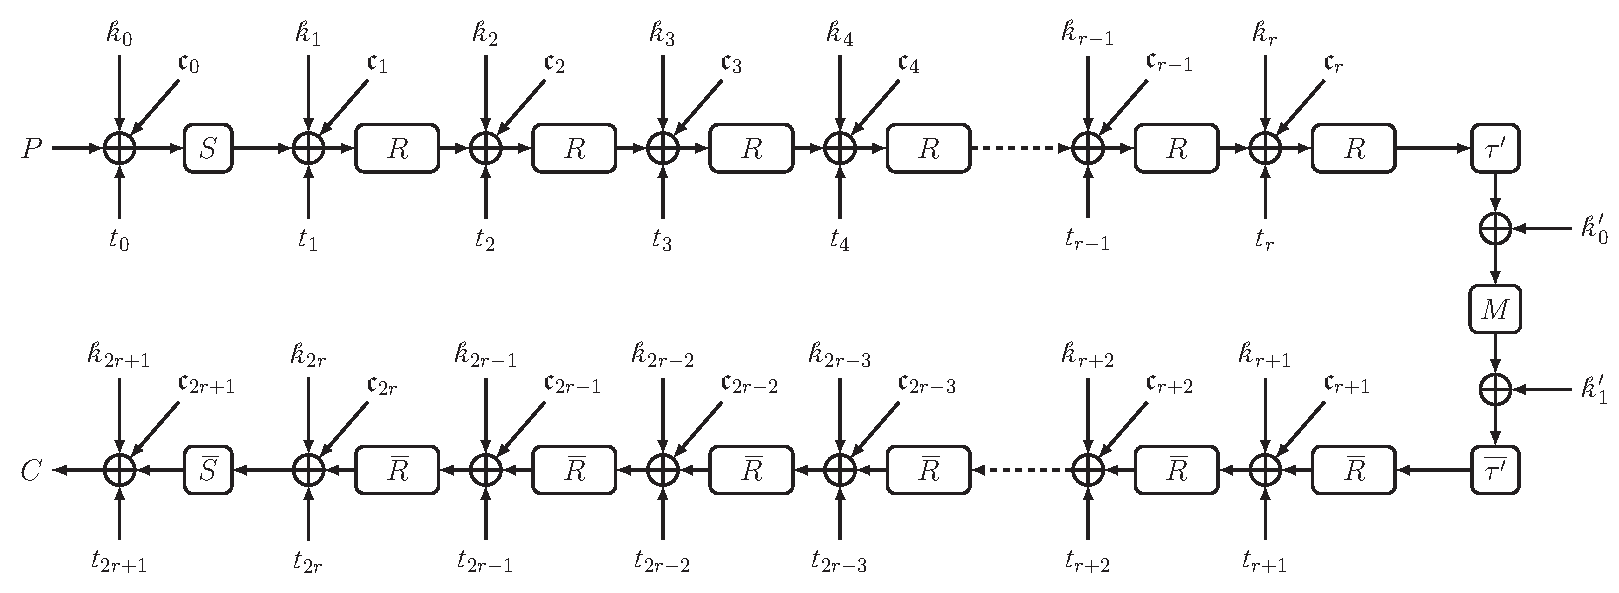
\includegraphics{./fig/QARMA-FAMILY.pdf}}

\scalebox{0.475}{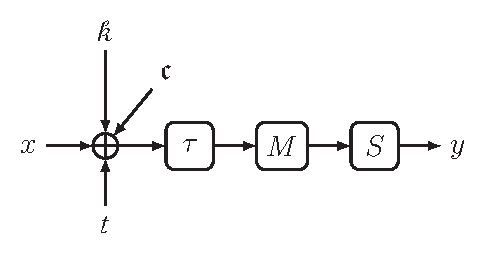
\includegraphics{./fig/QARMAv1-full-round.pdf}}
%%%%
\qquad\qquad%
\raisebox{23pt}[0pt][0pt]{\scalebox{0.7}{\(
    \begin{bmatrix}
        x_0  & x_1  & x_2  & x_3  \\
        x_4  & x_5  & x_6  & x_7  \\
        x_8  & x_9  & x_{10} & x_{11} \\
        x_{12} & x_{13} & x_{14} & x_{15}
    \end{bmatrix}
    \enspace
\)}}

\end{frame}

\begin{frame}
\frametitle{The S Layer and The M Layer}
\begin{align*}
    & \begin{bmatrix}
        x_0  & x_1  & x_2  & x_3  \\
        x_4  & x_5  & x_6  & x_7  \\
        x_8  & x_9  & x_{10} & x_{11} \\
        x_{12} & x_{13} & x_{14} & x_{15}
    \end{bmatrix}
    \xrightarrow{\quad \text{S Layer} \quad}
    \begin{bmatrix}
        s(x_0)  & s(x_1)  & s(x_2)  & s(x_3)  \\
        s(x_4)  & s(x_5)  & s(x_6)  & s(x_7)  \\
        s(x_8)  & s(x_9)  & s(x_{10}) & s(x_{11}) \\
        s(x_{12}) & s(x_{13}) & s(x_{14}) & s(x_{15})
    \end{bmatrix}, S: \mathbb{F}_2^4 \to \mathbb{F}_2^4  \\
    \pause
    \vspace{0.5cm}
    & \begin{bmatrix}
        x_0  & x_1  & x_2  & x_3  \\
        x_4  & x_5  & x_6  & x_7  \\
        x_8  & x_9  & x_{10} & x_{11} \\
        x_{12} & x_{13} & x_{14} & x_{15}
    \end{bmatrix}
    \xrightarrow{\quad \text{M Layer} \quad}
    \begin{bmatrix}
    \red {0}      & \red{\rho^a} & \red{\rho^b} & \red{\rho^c} \\
        \rho^c & 0      & \rho^a & \rho^b \\
        \rho^b & \rho^c & 0      & \rho^a \\
        \rho^a & \rho^b & \rho^c & 0
    \end{bmatrix}
    \otimes
    \begin{bmatrix}
        \blue{x_0}  & x_1  & x_2  & x_3  \\
        \blue{x_4}  & x_5  & x_6  & x_7  \\
        \blue{x_8}  & x_9  & x_{10} & x_{11} \\
        \blue{x_{12}} & x_{13} & x_{14} & x_{15}
    \end{bmatrix}
    \\
    &\text{Example: } (x_4 \lll a) \oplus (x_8 \lll b) \oplus (x_{12} \lll c)\\
    \pause
& M = M^{-1} \text{ over the ring } R_4 = \mathbb{F}_2[X]/(X^4 + 1)
\end{align*}

\end{frame}
\begin{frame}
\frametitle{State Mapped by $\tau$ to Different Columns}
\begin{align*}
    \centering
    \scalebox{1.2}{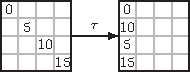
\includegraphics{./fig/column-number-map-0.pdf}} & \quad \quad
    \scalebox{1.2}{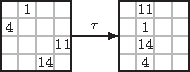
\includegraphics{./fig/column-number-map-1.pdf}}
    \\\\
    \scalebox{1.2}{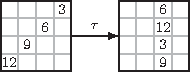
\includegraphics{./fig/column-number-map-2.pdf}} & \quad \quad
    \scalebox{1.2}{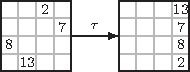
\includegraphics{./fig/column-number-map-3.pdf}}
\end{align*}
\end{frame}



\begin{frame}
\frametitle{\QARMAvi~\cite{DBLP:journals/tosc/Avanzi17}: The Tweakable Block Cipher}
\begin{enumerate}
\item \QARMAvi is a \red{reflection cipher}: \( E = F^{-1} \circ G \circ F: \mathbb{F}_2^{64} \to \mathbb{F}_2^{64} \)
\begin{figure}[t]
    \centering
    \scalebox{0.55}{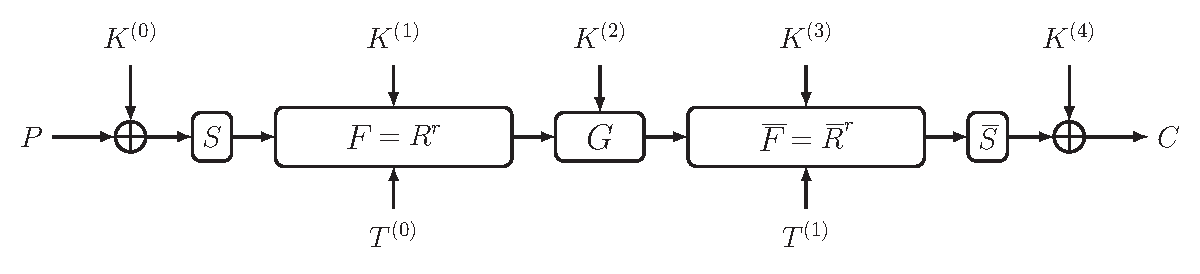
\includegraphics{./fig/structure.pdf}}
\end{figure}
\pause
\item \QARMAvi as the \acs{PAC} feature:
\begin{enumerate}
\item Pointer is used as the \red{"clamped"} plaintext input ( \red{\( 64-\mathtt{VA} \)} bits are set to \red{0})
\item Context is used as the tweak
\item The tag is the \red{"chopped"} ciphertext (attacker can only observe \red{\( 64 - \mathtt{VA} \)} bits)
\end{enumerate}
\end{enumerate}
\end{frame}

\begin{frame}
\frametitle{Summary of The Target}
\begin{enumerate}
\item \texttt{FEAT\_PACQARMA5} uses $\qarma{5}$, the 12-round version of \QARMAvi (100 GE) 
\pause
\item \red{\texttt{FEAT\_PACQARMA3} feature uses $\qarma{3}$, the 8-round \textsf{TBC} \QARMAvi (66 GE)}
\pause
\item Cryptanalysis of such a heavily round-reduced cipher is important
\pause
\item KPA: memory read gadgets are common, adversary can read signed pointers
\item \red{CPA}: JIT environments (e.g., JavaScript), allow to generate chosen pointer
\pause
\item Challenges in the cryptanalysis of \texttt{FEAT\_PACQARMA3}:
\begin{enumerate}
\item Clamping and chopping limits the differential characteristics we can use
\item Chopping the output bits creates high noise in key recovery
\end{enumerate}
\end{enumerate}
\end{frame}

\section{Differential Cryptanalysis of \texttt{FEAT\_PACQARMA3}}

\begin{frame}
    \frametitle{Cryptanalysis Perspective: \blue{Real} vs \green{Ideal} Distinguishing Game}
\centering
\textcolor{blue}{$\mathcal{E} \colon \mathcal{P} \times \mathcal{K} \to \mathcal{C}$} is a block cipher and \green{$\Pi$} is a random permutation

    \begin{center}
        \begin{tikzpicture}[transform shape, scale=1]
            \node[blockcipher1] (E) at (0,0) {$\mathcal{E}_{\kk}$};
            \node[blockcipher2] (P) at (4,0) {$\Pi$};
            \node               (O) at (2,-2) {};
            \node               (OO) at (2,-1.8) {$\mathcal{O}$};
            \node[left= 4cm of O]   (O1) {};
            \node[right=4cm of O]   (O2) {};
            \node[inner sep=0pt](A) at (2,-4){
\includegraphics[width=.125\textwidth]{./fig/think.png}};
            \draw[<->,dotted,thick] (A) -- (O);
            \draw[semithick,redd] (O1) -- (O2);
            \draw[dashed,semithick] (2,0.5) -- (OO);
            \node at (0.7, -2.5) {$\pp_1, \pp_2,...,\pp_d$};
            \node at (3.3, -2.5) {$\cc_1, \cc_2,...,\cc_d$};

            \draw[<->,dotted,thick] (0,-0.75) -- (OO) node [midway, above, sloped] {};
            \draw[<->,dotted,thick] (4,-0.75) -- (OO) node [midway, above, sloped] {};
        \end{tikzpicture}
    \end{center}
\end{frame}

\begin{frame}
\frametitle{Cryptanalysis Perspective}
    \centering
    \Large{\red{"Searching `Distinguisher'"} $|$ \blue{Key Recovery}}
\end{frame}

\begin{frame}
\frametitle{Differential Distinguisher}
\begin{center}
    \begin{tikzpicture}[every node/.style={font=\large}]
			\tikzset{
			    mynode/.style={rectangle,draw=black, thick, inner sep=1em, minimum size=3em, text centered, minimum width=2cm},
			    mynodep/.style={rectangle,text centered, minimum width=0.5cm, minimum height=1.1cm},
			    myarrow/.style={->, >=latex', shorten >=1pt, very thick}
			}
			\node[mynodep] (t1) {$\mathsf{X}_0$};
			\node[mynodep,right=0.5cm of t1] (Op1) {$\bigoplus$};
			\node[mynodep,right=0.5cm of Op1] (t1p) {$\mathsf{X}_1$};
			\node[mynodep,right=of t1p] (A1) {$= \Deltain$};

			\node[roundfunction, below=0.5cm of t1] (f) {$R$};
			\node[roundfunction, below=0.5cm of t1p] (fp) {$R$};

            \node[mynodep,below=0.5cm of f] (t2) {$\cc_0$};
			\node[mynodep,right=0.5cm of t2] (Op2) {$\bigoplus$};
			\node[mynodep,right=0.5cm of Op2] (t2p) {$\cc_1$};
			\node[mynodep,right=of t2p] (A2) {$\stackrel{?}{=} \Deltaout$};

			\draw[myarrow] (t1.south) -- (f.north);
			\draw[myarrow] (t1p.south) -- (fp.north);
			\draw[myarrow] (f.south) -- (t2.north);
			\draw[myarrow] (fp.south) -- (t2p.north);
		\end{tikzpicture}
\end{center}
{\Large $$\displaystyle \Pr\Big(R(\mathsf{X}) \oplus R(\mathsf{X} \oplus \Deltain) = \Deltaout \Big) = 2^{-q}, q \ll n$$}
\end{frame}


% Place this in your preamble or just before the content
\newcommand{\DistKeyRecoveryDiagram}{
\begin{tikzpicture}[node distance=1.2cm, every node/.style={font=\large}]
  % Nodes: P, R, F, XOR, C, K1, K2, E

  \draw[semithick, color = blue, rounded corners=1mm] (1,-0.7) rectangle (3, 2.8) node[above left] {Key Recovery};
  \draw[semithick, color = red, rounded corners=1mm] (4.5,-0.7) rectangle (6.5,2.8) node[above left] {Distinguisher};

  \node (P) {$\pp$};
  \node[roundfunction, right=of P, fill=blue!15] (F) {$F$};

  \node[right=1.25cm of F] (X) {};
  \node[above=0.2 of X] (Y) {$\mathsf{X}$};

  \node[roundfunction, right=2.5cm of F, fill=red!50] (R) {$R$};
  \node[right=of R] (C) {$\cc$};

  % Arrows for the main flow
  \draw[thick, -{Latex}] (P) -- (F);
  \draw[thick, -{Latex}] (F) -- (R);
  \draw[thick, -{Latex}] (R) -- (C);

  % K nodes and E node
  \node[above=1cm of F] (K1) {$\kk$};
  \node[above=1cm of R] (K2) {$\kk^{\prime}$};

  % K1 and K2 arrows
  \draw[thick, -{Latex}] (K1) -- (F);
  \draw[thick, -{Latex}] (K2) -- (R);
\end{tikzpicture}
}

\begin{frame}
\frametitle{Key Recovery Using Differential Distinguisher}
\begin{center}
    \DistKeyRecoveryDiagram
    \begin{itemize}
        \item $R(\cdot) = R_{r-1} \circ R_{r-2} \circ \cdots \circ R_{1} \circ R_{i}(\cdot)$
    \pause
\item $F(\pp_0, \kk) \oplus F(\pp_1, \kk) = \mathsf{X}_0 \oplus \mathsf{X}_1 = \Deltain \xrightarrow{2^{-q}} \Deltaout \text{, for the correct key } \kk$
    \end{itemize}
\end{center}
\end{frame}



\def\spelledoutemm{%
    \begin{pmatrix}
        0      & \rho^a & \rho^b & \rho^c \\
        \rho^c & 0      & \rho^a & \rho^b \\
        \rho^b & \rho^c & 0      & \rho^a \\
        \rho^a & \rho^b & \rho^c & 0
    \end{pmatrix}
}

\def\spelledoutemminverse{%
    \begin{pmatrix}
        0         & \rho^{-c} & \rho^{-b} & \rho^{-a} \\
        \rho^{-a} & 0         & \rho^{-c} & \rho^{-b} \\
        \rho^{-b} & \rho^{-a} & 0         & \rho^{-c} \\
        \rho^{-c} & \rho^{-b} & \rho^{-a} & 0
    \end{pmatrix}
}

% \begin{frame}
% \frametitle{\QARMAvi: The Round Function}
% \begin{figure}[!t]
%     \scalebox{0.599}{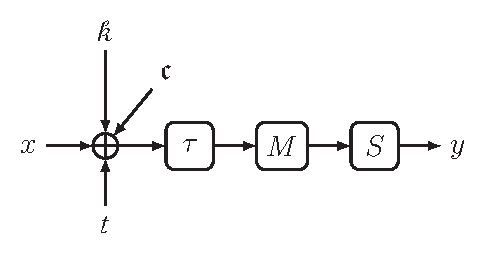
\includegraphics{./fig/QARMAv1-full-round.pdf}}
% \end{figure}
% \begin{enumerate}
% {\footnotesize
% \item \( M \) is an involutory Almost-MDS matrix
% \begin{displaymath}
%     M = \mathrm{circ}(0, \rho^1, \rho^2, \rho^1) =
%     \spelledoutemm
%     \enspace 
% \end{displaymath}

% \item \( \tau = [\,0, 11, 6, 13, 10, 1, 12, 7, 5, 14, 3, 8, 15, 4, 9, 2\,]\)
% \item \( \sigma_0 := [\, 0,14,2,10,9,15,8,11,6,4,3,7,13,12,1,5\,] \)
% }
% \end{enumerate}

% \end{frame}



\begin{frame}
\frametitle{Differential Attack on a Clamped and Chopped Cipher}
\begin{figure}[!t]
    \centering
    \scalebox{1}{%
        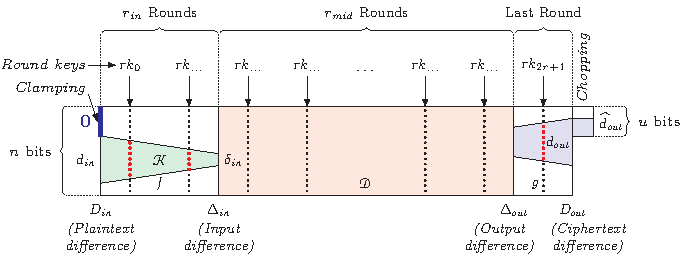
\includegraphics{./fig/keyRecovery-frontonly-shorterback-no-bottom.pdf}}%
\end{figure}

\begin{itemize}
{\footnotesize
\item No difference, and no control over the \red{clamped} bits
\item Output is \red{chopped}, the adversary can observe only \red{$u$} bits
\pause
\item \green{$q \stackrel{\triangle}{=} - \log_2(\Pr[\Deltain \rightarrow \Deltaout])$}
}
\end{itemize}
\end{frame}

\begin{frame}
\frametitle{An Example of $\mathtt{VA} = 52$}
\begin{align*}
    \!\!\scalebox{0.666}{%
        \begin{tikzpicture}
             \node[anchor=north west] at (0,0) {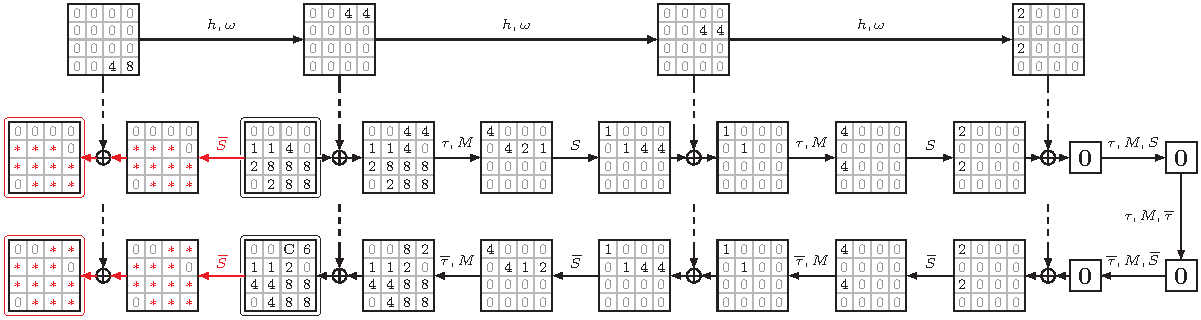
\includegraphics{./fig/qarmav1_r_333_t_1_KR_wf_0_zc_4_W_24.pdf}};
            \node[inner sep=0pt,fill=white] at (.425,-2.35)  {\small\textcolor{blue}{{\bfseries 0}}};
            \node[inner sep=0pt,fill=white] at (.725,-2.35)  {\small\textcolor{blue}{{\bfseries 0}}};
            \node[inner sep=0pt,fill=white] at (1.025,-2.35) {\small\textcolor{blue}{{\bfseries 0}}};
            \draw[color=blue,rounded corners=1.667pt,semithick,small cross line] (0.31,-4.235) -- (1.14,-4.235) -- (1.14,-4.465) -- (0.31,-4.465) -- cycle;
        \end{tikzpicture}\!\!\!}
    \raisetag{3.55cm}
\end{align*}


\centering
$\din = 4 \times 10 = 40, u = 12, \hatdout = 4, q = 12, \text{ i.e., } \Pr[\Deltain \rightarrow \Deltaout] = 2^{-12}$
\end{frame}

\begin{frame}
\frametitle{Key Recovery Goal}
    \centering
    \scalebox{0.64}{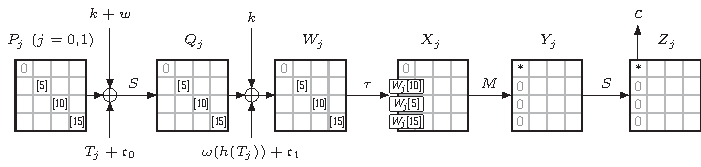
\includegraphics{./fig/through-one-half-rounds-1.pdf}}%

    \medskip
    \centering
    The 128-bit master key is \red{\( K = w \Vert k \)} and let, \green{\( k' = M(\tau(k)) \)}

    \medskip
    \centering
    \scalebox{0.64}{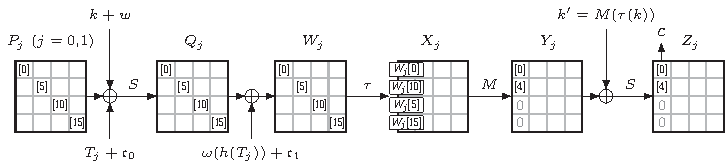
\includegraphics{./fig/through-one-half-rounds-key-add-shifted-two-cells.pdf}}%
    
    \pause
    \centering
    \begin{description}
    \item [\red{Data}:] $\leq 2^{30}$ chosen plaintext-tweak pairs
    \item [\red{Time}:] $\leq 2^{64} $ (\red{Break}) and  $\leq 2^{80} $ (\blue{Warning})
    \end{description}

\end{frame}

\begin{frame}
\frametitle{Overview of the Attacks}

\begin{block}{Structures}
    {\footnotesize \( \calS \) : \( \calS_0, \calS_1 \subseteq \mathbb{F}_2^{n} \times \mathbb{F}_2^{n_t} \) and \( \calS_1=(0,\mathbf{t}_0)+\calS_0 \). \blue{ \( |\calS_i| = 2^{\din}, |\calS| = 2^{2 \din} \) } with data complexity \red{$2^{\din + 1}$}}
\end{block}
\pause
\begin{block}{Pair Sieving}
  \centering%
  \scalebox{0.8}{%
  \begin{minipage}{\linewidth}
    \vspace{-6pt}%
    \begingroup
    \begin{algorithm}[H]
      \begin{algorithmic}[1]
        \For{\( \big((P_0, T_0), (P_1, T_1)\big) \in \calS_0 \times \calS_1 \)}
            \If{\( \calE_{T_0,K}(P_0) + \calE_{T_1,K}(P_1) \in \Dout \)}
               \( \calC = \calC \cup \big((P_0, T_0, C_0), (P_1, T_1, C_1)\big) \)
            \EndIf
        \EndFor
      \end{algorithmic}
    \end{algorithm}
    \endgroup
  \end{minipage}%
 }
\end{block}
\pause

\begin{block}{Guess-and-Filter}
  \centering%
  \scalebox{0.8}{%
  \begin{minipage}{\linewidth}
    \vspace{-6pt}%
    \begingroup
    \begin{algorithm}[H]
      \begin{algorithmic}[1]
      \AlgoState Prepare a dictionary \( \chi \) associated with the elements \( \keyguess\in\langle\Kbits\rangle \) (\red{AVL trees})
            \For{\( \big((P_0, T_0, C_0), (P_1, T_1, C_1)\big) \in \calC \)}
                \For{\( \keyguess\in\langle\Kbits\rangle \)}
                  \If{\( \calf_{\keyguess} (\theinput0)+\calf_{\keyguess}(\theinput1)\in\Deltain \)}
                    \label{KRP:loop}
                    {\vphantom{\( 2^{2^2} \)}\( \chi(\keyguess) = \chi(\keyguess) + 1 \)}
                  \EndIf
                \EndFor%
            \EndFor%
      \end{algorithmic}
    \end{algorithm}
    \endgroup
  \end{minipage}%
 }
\end{block}
\end{frame}

\begin{frame}
\frametitle{Attack on $\mathtt{VA} = 56$ (Char. $1$)}
\begin{align*}
    \!\!\scalebox{0.6}{%
        \begin{tikzpicture}
        \node[anchor=north west] at (0,0) {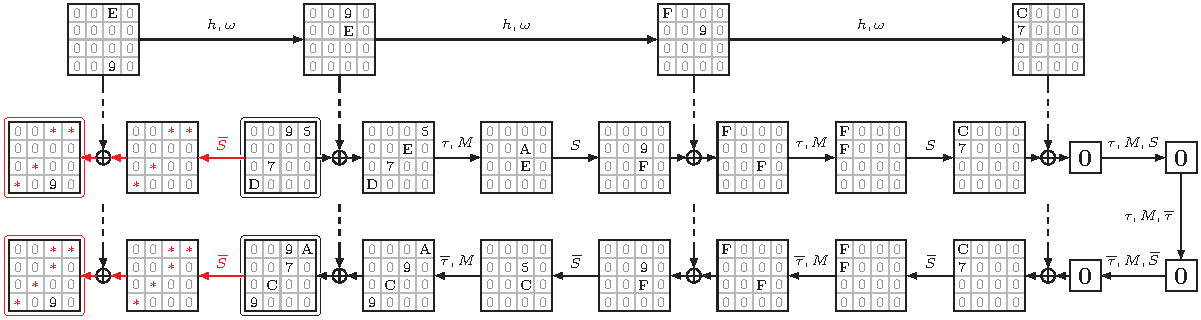
\includegraphics{./fig/qarmav1_r_333_t_1_KR_zc_0.pdf}};
            \node[inner sep=0pt,fill=white] at (.425,-2.35) {\small\textcolor{blue}{{\bfseries 0}}};
            \node[inner sep=0pt,fill=white] at (.725,-2.35) {\small\textcolor{blue}{{\bfseries 0}}};
            \draw[color=blue,rounded corners=1.667pt,semithick,small cross line] (0.31,-4.235) -- (0.84,-4.235) -- (0.84,-4.465) -- (0.31,-4.465) -- cycle;
        \end{tikzpicture}\!\!\!}
    \raisetag{3.55cm}
\end{align*}

\pause
\begin{description}
\item [\green{0.5R} Attack:] Recover the \( 16 \) key bits \( (k+w)[\{2, 3,9,12\}] \)
\pause
% {\footnotesize
% \begin{itemize}
% \item \( \Deltain[i] = S\big(P_0[i]+T_0[i]+(k+w)[i]\big) + S\big(P_1[i]+T_1[i]+(k+w)[i]\big), i \in \{2,3,9,12\}\)
% \end{itemize}
% }
% \pause
\item [\red{Peeling}:] Recover the \( 8 \) key bits \( k'[\{6,10\}] \) using \( (k+w)[\{6\}] \)
\end{description}

\end{frame}

\begin{frame}
\frametitle{Attack on $\mathtt{VA} = 56$ (Char. $2$)}

\!\!\scalebox{0.6}{%
        \begin{tikzpicture}
\node[anchor=north west] at (0,0) {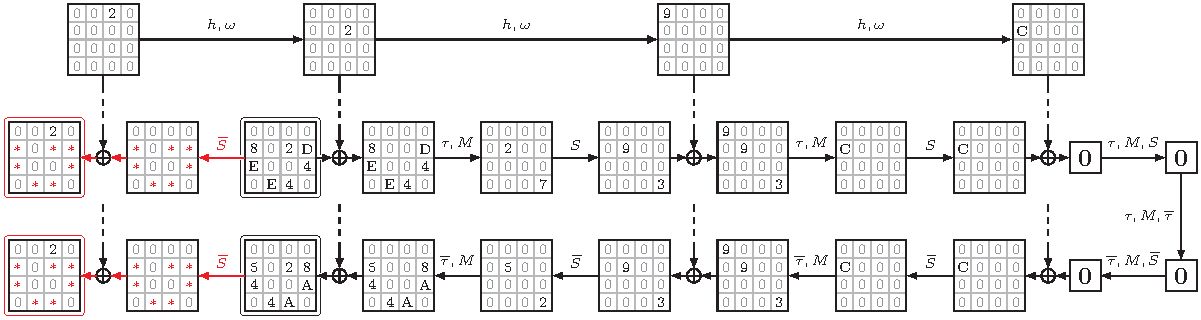
\includegraphics{./fig/qarmav1_r_333_t_1_KR_zc_2_(4,6,7,8,11,13,14)_44_ASSERT_FT2r0=0b0010.pdf}};
            \node[inner sep=0pt,fill=white] at (.425,-2.35) {\small\textcolor{blue}{{\bfseries 0}}};
            \node[inner sep=0pt,fill=white] at (.725,-2.35) {\small\textcolor{blue}{{\bfseries 0}}};
            \draw[color=blue,rounded corners=1.667pt,semithick,small cross line] (0.31,-4.235) -- (0.84,-4.235) -- (0.84,-4.465) -- (0.31,-4.465) -- cycle;
        \end{tikzpicture}\!\!\!}
    \raisetag{3.55cm}

\begin{description}
\item [\green{0.5R} Attack:] Recover the \( 28 \) key bits \( (k+w)[\{4, 6, 7, 8, 11, 13, 14\}] \)
\item [\red{Peeling}:] Recover the \( 8 \) key bits \( k'[\{5, 15\}] \) by guessing \( (k+w)[\{1\}] \)
\end{description}
\end{frame}

\begin{frame}
\frametitle{Attack on $\mathtt{VA} = 56$ (Char. $3$)}
\begin{align*}
    \!\!\scalebox{0.6}{%
        \begin{tikzpicture}
        \node[anchor=north west] at (0,0) {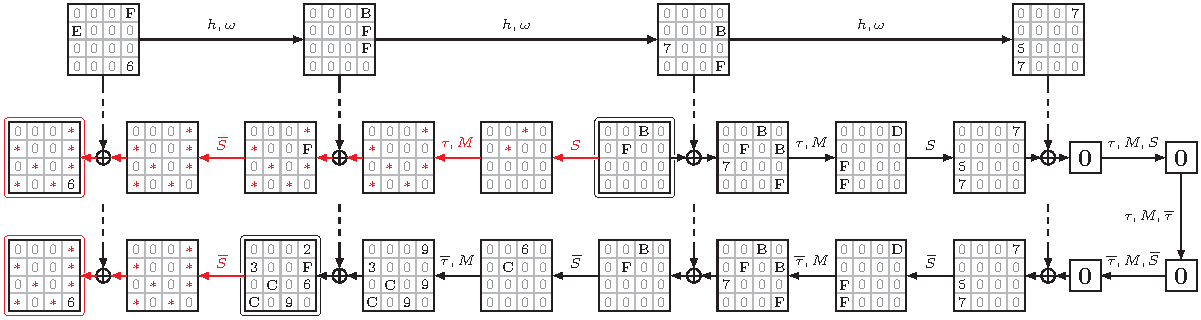
\includegraphics{./fig/qarmav1_r_323_t_1_KR_zc_3_(3,4,7,9,11,12,14)_50.pdf}};
            \node[inner sep=0pt,fill=white] at (.425,-2.35)  {\small\textcolor{blue}{{\bfseries 0}}};
            \node[inner sep=0pt,fill=white] at (.725,-2.35)  {\small\textcolor{blue}{{\bfseries 0}}};
            \draw[color=blue,rounded corners=1.667pt,semithick,small cross line] (0.31,-4.235) -- (0.84,-4.235) -- (0.84,-4.465) -- (0.31,-4.465) -- cycle;
        \end{tikzpicture}\!\!\!}
    \raisetag{3.55cm}
\end{align*}

\begin{description}
\item [\red{Peeling}:] Recover the \( 4 \) key bits \( k'[2] \) using \( (k+w)[\{3,9,12\}] \)
\end{description}

\end{frame}

\begin{frame}
\frametitle{Summarized Attack Results on $\mathtt{VA} = 56$}
\begingroup
\setlength\arraycolsep{3pt}
\begin{DIFnomarkup}
{\Large 
    \begin{equation*}
        \label{eq:mat2}
        (k+w) \gets
        \begin{bmatrix}
            b  & 1  & 1 & 2 \\
            1  & b  & 1 & 1 \\
            1  & 2  & b & 1 \\
            2  & 1  & 1 & b
        \end{bmatrix}
        \quad\text{and}\quad
        %\hspace{1cm}
        k' \gets
        \begin{bmatrix}
            b & b & 3 & b \\
            b & 1 & 2 & b \\
            b & b & 2 & b \\
            b & b & b & 1
        \end{bmatrix}
        \enspace
    \end{equation*}
}
\end{DIFnomarkup}
\endgroup

\begin{description}
    \item[\red{Time Complexity}] \( \approx 2^{60}\,\costq \) (dominated by the brute force step)
    \item[\textcolor{green}{Data Complexity}] \( \approx 2^{25} \) Chosen Plaintexts
\end{description}

\end{frame}


\section{Data Complexity, Time Complexity and Success Probability}
\begin{frame}
\frametitle{An Example of 0.5R Attack on $\mathtt{VA} = 56$}
\begin{align*}
    \!\!\scalebox{0.7}{%
        \begin{tikzpicture}
            \node[anchor=north west] at (0,0) {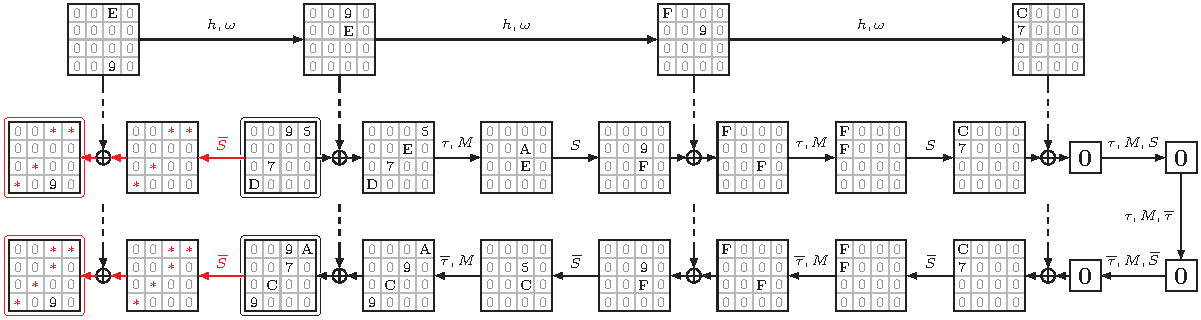
\includegraphics{./fig/qarmav1_r_333_t_1_KR_zc_0.pdf}};
            \node[inner sep=0pt,fill=white] at (.425,-2.35) {\small\textcolor{blue}{{\bfseries 0}}};
            \node[inner sep=0pt,fill=white] at (.725,-2.35) {\small\textcolor{blue}{{\bfseries 0}}};
            \draw[color=blue,rounded corners=1.667pt,semithick,small cross line] (0.31,-4.235) -- (0.84,-4.235) -- (0.84,-4.465) -- (0.31,-4.465) -- cycle;
        \end{tikzpicture}\!\!\!}
    \raisetag{3.55cm}
\end{align*}
\end{frame}

\begin{frame}
\frametitle{An Example of 0.5R Attack on $\mathtt{VA} = 56$}
\begin{columns}[t]
\begin{column}{0.5\textwidth}
\begin{align*}
    \!\!\scalebox{0.35}{%
        \begin{tikzpicture}
            \node[anchor=north west] at (0,0) {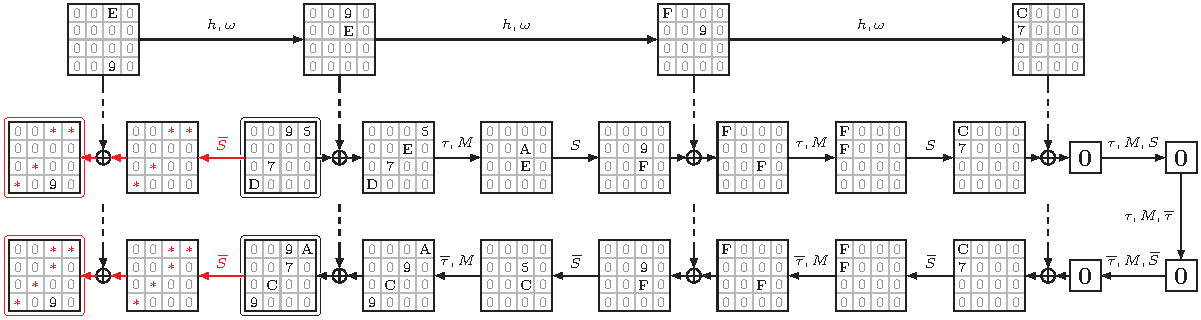
\includegraphics{./fig/qarmav1_r_333_t_1_KR_zc_0.pdf}};
            \node[inner sep=0pt,fill=white] at (.425,-2.35) {\small\textcolor{blue}{{\bfseries 0}}};
            \node[inner sep=0pt,fill=white] at (.725,-2.35) {\small\textcolor{blue}{{\bfseries 0}}};
            \draw[color=blue,rounded corners=1.667pt,semithick,small cross line] (0.31,-4.235) -- (0.84,-4.235) -- (0.84,-4.465) -- (0.31,-4.465) -- cycle;
        \end{tikzpicture}\!\!\!}
    \raisetag{3.55cm}
\end{align*}
\begin{enumerate}
\item We have \( q = 10 \), \( \din=16 \)
\item \( 16 \) key bits \( (k+w)[\{2, 3,9,12\}] \)
\item $u - \hatdout = 8$
\end{enumerate}
\end{column}
\pause
\begin{column}{0.5\textwidth}
\begin{block}{$N$: $\#$pairs satisfying \red{\( \Deltain \)}??}
\pause
{\footnotesize \green{$R:$} Counters Corr. to \green{``Right keys''}}\\
{\footnotesize \red{$W:$} Counters Corr. to \red{``Wrong keys''}}
\pause
\begin{enumerate}
{\footnotesize
\item  \red{\(W \sim \text{Poisson}\big(N \cdot 2^{-8}\big) \)}
\item  \green{\(R \sim \text{Poisson}(N\cdot(2^{-8}+2^{-10})) \)}
\item  \(\sigma = \sqrt{N \cdot 2^{-8} \big(1-2^{-8}\big)}\)
}
\end{enumerate}


\end{block}
\end{column}
\end{columns}

\end{frame}

\begin{frame}
\frametitle{Counters Corresponding to Right vs Wrong Keys}
\begin{figure}
    \scalebox{0.5}{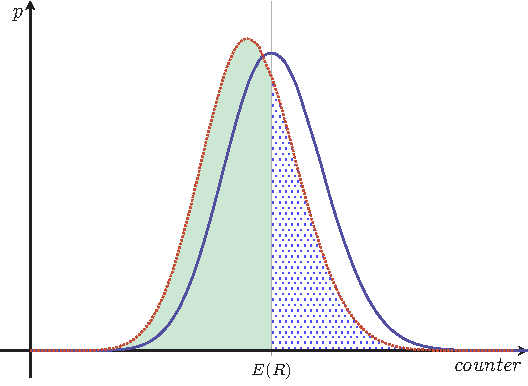
\includegraphics{./fig/success-probability-1-tight.pdf}} \quad
    \scalebox{0.5}{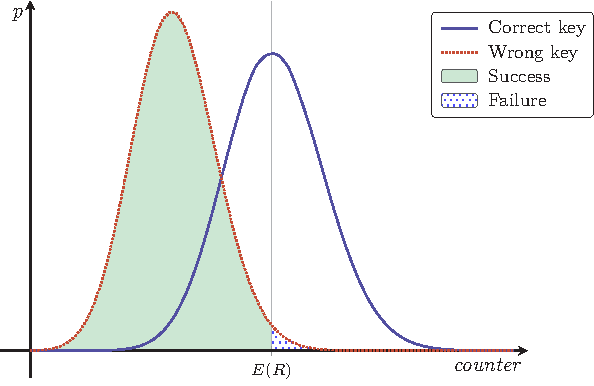
\includegraphics{./fig/success-probability-1-wide.pdf}}
\end{figure}
\pause
\begin{enumerate}
\item {\footnotesize $E[R] - E[W] \geq \gamma \sigma \implies N\cdot\left(2^{-q}+2^{-u+\hatdout}\right) - N \cdot\left(  2^{-u+\hatdout} \right) \geq \gamma \sqrt{N \cdot 2^{-u+\hatdout}\cdot \left(1-2^{-u+\hatdout}\right)} $}
\pause
\item {\footnotesize Success Probability: $\displaystyle \Bigg(\sum_{a \leq E(R)} \Pr[W = a] \Bigg)^{\nu-1}$, where $\nu$ is the $\#$possible keys}
\end{enumerate}
\end{frame}


\begin{frame}
\frametitle{An Example of 0.5R Attack on $\mathtt{VA} = 56$}
\begin{columns}[t]
\begin{column}{0.4\textwidth}
\begin{figure}
\scalebox{0.4}{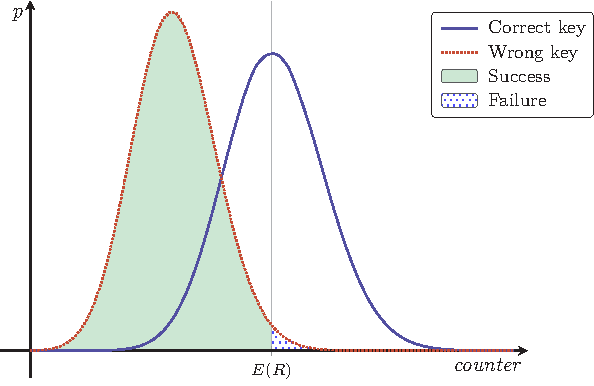
\includegraphics{./fig/success-probability-1-wide.pdf}}\\
\vfill
\hspace{-0.45cm}\scalebox{0.4}{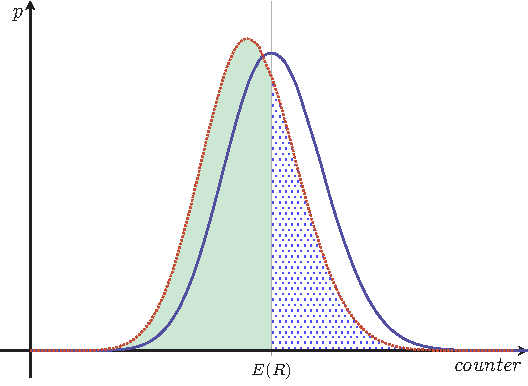
\includegraphics{./fig/success-probability-1-tight.pdf}}
\end{figure}
\end{column}

\begin{column}{0.55\textwidth}
\begin{block}{$N$: $\#$pairs satisfying \( \Deltain \)??}
\begin{enumerate}

{\footnotesize
\item We have \( q = 10 \), \( \din=16 \)
\item \( 16 \) key bits \( (k+w)[\{2, 3,9,12\}] \), $\nu = 2^{16}$
\pause
\item $N\cdot 2^{-10} \geq \gamma \sqrt{N\cdot 2^{-8} \big(1-2^{-8}\big)}$
\item  \(\gamma = 8 \) gives \red{\( N \approx 2^{18} \)}
\pause
\item So we need $2^2$ structures of size \( 2^{16} \)
\item Data Complexity: \( 2 \times 2^2 \times 2^{16} = 2^{19} \)
\pause
\item Sieved Pairs: $L \approx 2^{26}$
\item Time Complexity: \( 2^{27} \costq\)
}
\end{enumerate}
\end{block}

\end{column}
\end{columns}

\end{frame}

\section{Experimental Verification}
\begin{frame}
\frametitle{Experimental Verification}
\let\ofhundred\relax
{\footnotesize 
\begin{enumerate}
\item \( \bar{h}_i \): $\#$ pairs that satisfy $\Dout$ in the \( i \)-th experiment and random noise \( \eta = N \cdot 2^{-u + \hatdout} \)
\item \( \bar{q} = - \log_2( \textrm{Mean}(\bar{h}_i-\eta) /N ) \)
\item If \( \bar{h}_i - \eta > (1/2)\gamma \sigma \), we consider the experiment to have been successful
\end{enumerate}
}
%\smash{\scalebox{0.8}{\rotatebox[origin=c]{90}{\(u - \hatdout\)}}}
\begin{table}[!t]
    \centering%
    %\renewcommand{\arraystretch}{1.12}
    \begingroup
    \addtolength{\tabcolsep}{-0.15em}
    % \resizebox{\linewidth}{!}{
    \scalebox{0.77}[0.77]{

\begin{tabular}{cccc|
>{\columncolor[HTML]{C0C0C0}}r 
>{\columncolor[HTML]{C0C0C0}}c 
>{\columncolor[HTML]{C0C0C0}}l |ccc}
 &  &  &  & \multicolumn{3}{c|}{\cellcolor[HTML]{C0C0C0}$\bar{h}_i - \eta$} &  &  & Successes \\
\multirow{-2}{*}{Char.} & \multirow{-2}{*}{\smash{\scalebox{0.8}{\rotatebox[origin=c]{90}{\(u - \hatdout\)}}}} & \multirow{-2}{*}{$N$} & \multirow{-2}{*}{$\sigma$} & Mean & $\pm$ & S.D. & \multirow{-2}{*}{$q$} & \multirow{-2}{*}{$\bar{q}$} & /100 trials \\ \hline
1 & 8 & $2^{14}$ & 7.98 & 64.11 & $\pm$ & 11.69 & 7.98 & 8.00 & 100 \\
2 & 8 & $2^{18}$ & 31.94 & 256.19 & $\pm$ & 32.40 & 10.01 & 10.00 & 100 \\
3 & 12 & $2^{18}$ & 7.99 & 63.80 & $\pm$ & 11.50 & 12.01 & 12.00 & 100 \\
{\color[HTML]{FE0000} 4} & {\color[HTML]{FE0000} 8} & {\color[HTML]{FE0000} $2^{22}$} & {\color[HTML]{FE0000} 127.75} & {\color[HTML]{FE0000} 1022.33} & {\color[HTML]{FE0000} $\pm$} & {\color[HTML]{FE0000} 1832.27} & {\color[HTML]{FE0000} 12.00} & {\color[HTML]{FE0000} 12.00} & {\color[HTML]{FE0000} 27} \\
{\color[HTML]{3166FF} $4^{\star}$} & {\color[HTML]{3166FF} 8} & {\color[HTML]{3166FF} $2^{18}$} & {\color[HTML]{3166FF} 31.93} & {\color[HTML]{3166FF} 258.32} & \multicolumn{1}{l}{\cellcolor[HTML]{C0C0C0}{\color[HTML]{3166FF} $\pm$}} & {\color[HTML]{3166FF} 39.27} & {\color[HTML]{3166FF} 10.00} & {\color[HTML]{3166FF} 9.98} & {\color[HTML]{3166FF} 100} \\
{\color[HTML]{FE0000} 5} & {\color[HTML]{FE0000} 12} & {\color[HTML]{FE0000} $2^{29}$} & {\color[HTML]{FE0000} 361.99} & {\color[HTML]{FE0000} 2128.71} & {\color[HTML]{FE0000} $\pm$} & {\color[HTML]{FE0000} 2075.29} & {\color[HTML]{FE0000} 18.00} & {\color[HTML]{FE0000} 17.94} & {\color[HTML]{FE0000} 53} \\
{\color[HTML]{3166FF} $5^{\star}$} & {\color[HTML]{3166FF} 12} & {\color[HTML]{3166FF} $2^{27}$} & {\color[HTML]{3166FF} 181.00} & {\color[HTML]{3166FF} 1026.25} & \multicolumn{1}{l}{\cellcolor[HTML]{C0C0C0}{\color[HTML]{3166FF} $\pm$}} & {\color[HTML]{3166FF} 174.94} & {\color[HTML]{3166FF} 17.00} & {\color[HTML]{3166FF} 17.00} & {\color[HTML]{3166FF} 100} \\
6 & 16 & $2^{31}$ & 181.02 & 1028.42 & $\pm$ & 176.56 & 21.00 & 20.99 & 100 \\
7 & 4 & $2^{33}$ & 5781.29 & 33324.88 & $\pm$ & 6337.25 & 18.00 & 17.97 & {\color[HTML]{333333} 100} \\ \hline
\end{tabular}
    }
    \endgroup
\end{table}
\end{frame}


\begin{frame}
\frametitle{Conditional Characteristic (Char. \red{4})}
\begin{align*}
    \!\!\scalebox{0.7}{%
        \begin{tikzpicture}
            \node[anchor=north west] at (0,0) {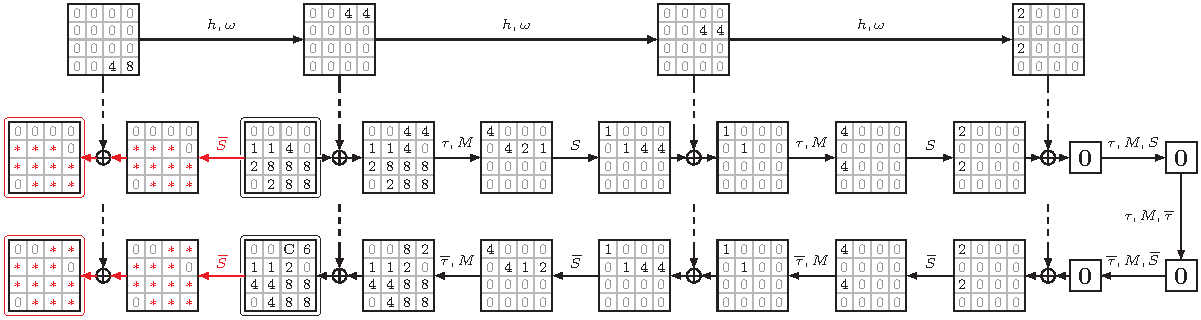
\includegraphics{./fig/qarmav1_r_333_t_1_KR_wf_0_zc_4_W_24.pdf}};
            \node[inner sep=0pt,fill=white] at (.425,-2.35)  {\small\textcolor{blue}{{\bfseries 0}}};
            \node[inner sep=0pt,fill=white] at (.725,-2.35)  {\small\textcolor{blue}{{\bfseries 0}}};
            \node[inner sep=0pt,fill=white] at (1.025,-2.35) {\small\textcolor{blue}{{\bfseries 0}}};
            \draw[color=blue,rounded corners=1.667pt,semithick,small cross line] (0.31,-4.235) -- (1.14,-4.235) -- (1.14,-4.465) -- (0.31,-4.465) -- cycle;
        \end{tikzpicture}\!\!\!}
    \raisetag{3.55cm}
\end{align*}
\end{frame}

\begin{frame}
\frametitle{Conditional Characteristic (Char. \red{4})}
\begin{figure}[!t]
    \centering
    \scalebox{0.7}{%
        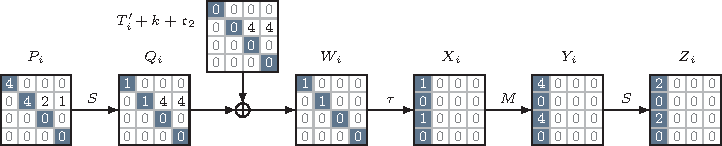
\includegraphics{./fig/third-round-dependencies-2.pdf}}%
\end{figure}%
\pause
\begin{displaymath}
    \begin{aligned}
        \Delta_P \to \Delta_Q & \Rightarrow \calA = \{ x: S(x + \texttt{4}) + S(x) =\texttt{1}\}=\{\texttt{1}, \texttt{3}, \texttt{5}, \texttt{7}\}              \\
        \Delta_Y \to \Delta_Z & \Rightarrow \calB = \{ x: S(x + \texttt{4}) + S(x) =\texttt{2}\}=\{\texttt{10}, \texttt{11}, \texttt{14}, \texttt{15}\} \\
\pause
& (T_i' + k + \RC_2)[5] + (T_i' + k + \RC_2)[0] \in \{ \texttt{0}, \texttt{1}, \texttt{4}, \texttt{5} \}
    \end{aligned}
\end{displaymath}
\pause
\begin{equation*}
     \begin{cases}
        T_i[2][2] \hphantom{{} + T_i[2][0]} + T_i[5][2] \hphantom{{} +T_i[2][1]} + (k+\RC_2)[0][1] + (k+\RC_2)[5][1] = 0 \\[2pt]
        T_i[2][0] + T_i[2][1] + T_i[5][0] + T_i[5][1] + (k+\RC_2)[0][3] + (k+\RC_2)[5][3] = 0  \enspace
     \end{cases}
\end{equation*}
\pause
{\small \red{AutoDiVer: Automatically Verifying Differential Characteristics and Learning Key Conditions.} IACR Trans. Symmetric Cryptol., 2025(1):471–514, 2025}
\end{frame}

\section{Results}

\begin{frame}
\frametitle{Results}
\begin{table}[t]
    \normalsize%
    \centering%
    \begingroup%
    \addtolength{\tabcolsep}{-0.125em}
    % \resizebox{\textwidth}{!}{
    \scalebox{0.845}[0.875]{%
        \begin{tabular}{c@{}cccccl}
            \toprule
            & Rounds       & \texttt{VA}~\&& \multicolumn{3}{c}{\raisebox{-1pt}{\braceA{0.65}{0.75pt}} Attack Complexity \raisebox{-1pt}{\braceB{0.65}{0.75pt}}} & \middleoftworows{Technique} \\
            & attacked           & Profile & Data          & Time               & Memory                 &                                 \\
            \midrule
            & \(4+4\)    & \itshape \red{56 (A)} & \(2^{25}\) CP      & \(2^{60}\)    & \( 2^{28.98} \)        & {\itshape RT Diff.} \\
            & \(4+4\)    & \itshape \red{ 52 (A) } & \(2^{25.3}\) CP    & \(2^{55}\)    & \( 2^{28.94} \)        & {\itshape RT Diff.}             \\
            & \(4+4\)    & \itshape \red{ 48 (A) } & \(2^{28}\) CP      & \(2^{60}\)    & \( 2^{40.83} \)        & \blue{{\itshape RT Mult.~Diff.}} \\
            & \(4+4\)    & \itshape \red{ 44 (A) }& \(2^{31.19}\) CP   & \( 2^{68} \)  & \( 2^{31.67} \)        & {\itshape RT Diff.}             \\
            & \(4+4\)    & \itshape \blue{40 (A)} & \(2^{37.5}\) CP    & \( 2^{76} \)  & \( 2^{38.82} \)        & {\itshape RT Diff.}             \\
            & \(4+4\)    & \itshape \blue{ 36 (A)} & \(2^{33.7}\) CP    & \( 2^{76} \)  & \( 2^{35.02} \)        & {\itshape RT Diff.}             \\
            & \(4+4\)    & \itshape \green{32 (A)} & \(2^{42}\) CP      & \( 2^{76} \)  & \( 2^{44.32} \)        & {\itshape RT Diff.}             \\
            & \(4+4\)    & \itshape \green{32 (M)} & \(2^{45}\) CP      & \( 2^{76} \)  & \( 2^{46.32} \)        & {\itshape RT Diff.}             \\[6pt] %\graymidrule
            \bottomrule
            \end{tabular}%
            }
    \endgroup%
\end{table}
\centering
*RT: Related-Tweak
\end{frame}

\begin{frame}
\frametitle{Conclusion}

\begin{enumerate}
    \item Practical attacks on \qarma{3} used in \texttt{FEAT\_PACQARMA3}
    \begin{enumerate}
        \item Despite (\red{clamping}, \red{chopping}), our attacks outperform previous ones on \qarma{3}
        \item Versions with \texttt{VA} = \red{44, 48, 52}, and 56 do not meet the expected security level
    \end{enumerate}
    \pause
    \item Finding good characteristics is challenging in \red{clamped} and \red{chopped} ciphers
    \begin{enumerate}
        \item We designed a bit-wise model of the $\rmid$ middle rounds as a program for \textsf{STP}
        \item Maximizing the prob. of a characteristic ($2^{-p}$) alone is insufficient $\rightarrow p+\din$
        \item We observed strong \red{clustering} effects.
    \end{enumerate}
    \pause
    \item Future directions
    \begin{enumerate}
        \item Our results do not directly translate to practical breaks of the \ac{PAC} \emph{feature}
        \item Investigating practical constraints that hinder real-world attacks
        \item Extending our framework to analyze the security of \(\mbox{\QARMAvii}\) within \ac{PAC} \emph{feature}
    \end{enumerate}
\end{enumerate}
\end{frame}

\begin{frame}
    \begin{columns}[t]
        \begin{column}{0.50\linewidth}
            \begin{figure}[!h]
                \centering
                
\includegraphics[width=5.7cm]{./img/qr_with_logo.png}
            \end{figure}
        \end{column}
        \pause
        \begin{column}{0.50\linewidth}
            \begin{center}
                {\huge {\color{red} Thank You} for your attention!} \\ \Large Any questions?
            \end{center}
        \end{column}
    \end{columns}
\end{frame}

\bibliographystyle{alpha}
\bibliography{../bibliography.bib}

\end{document}
